\section{External Interface Requirements}
\label{sec:external_interface_requirements}%

\subsection{User Interfaces}
\label{subsec:user_interfaces}%
The eMALL’s user interfaces are a website and a mobile application;
the first is developed to be used mainly by CPOs with a dedicated login section for businesses but can be used by EVDs too.
The mobile application is available for Android and iOS and provides an enhanced experience as compared to the website
since it offers users personalized suggestions based on their location.
The website and the app should be easy to use since they will be used mostly by middle-aged users,
who might not always be familiar with the technology.
A “quick booking” section dedicated to facilitating the booking process might be included,
for those EVDs who are used to booking a charge at the same charging station (based on suggestions given by AI).

\subsection{Hardware Interfaces}
\label{subsec:hardware_interfaces}%
The system only requires a smartphone or computer with an internet connection and web browser to access websites or mobile applications.
Furthermore, eMALL communicates with the EV through its company's API to get the current battery level, the charging state,
so if it is plugged in and if it is charging, and the number of routable kilometers obtained on the current battery level.
To access personalized suggestions, based on EV’s position, the device in use has to be able to detect its location with a GPS or Glonass localization system.

\subsection{Software Interfaces}
\label{subsec:software_interfaces}%
The following list describes the required software interfaces that the \verb|eMALL| system uses:
\begin{itemize}
    \item \textbf{CPMS and Charging Points.} The CPMS that is offered to the CPO communicates with the charging points
    through their API\@.
    Thanks to it, the system can manage the charging session, given the possibility of starting and stopping it or set
    the power supply to be given to each connected EV\@.
    Another significant functionality is the diagnostic of the charging point:
    a CPO can reboot its charging spots, can get their log, and can update their firmware.
    %TODO: Does it make sense to put an example of an external system
    \item \textbf{eMALL and EVs.} The eMALL system communicates with the EVs registered by the EVD\@.
    As explained in the domain assumption section, we suppose that there is a third-party system that offers its API
    so to get the status of the battery of the EV\@.
    %An example of a system that provides these features is Smartcar,
    %which is already used by companies like AmpUp or BeCharge to remotely retrieve the battery level and remaining range of the EVs.
    \item \textbf{CPMS and DSOs.} The CPMSs offered to the CPO communicate with the DSOs through their APIs.
    CPOs can get selling prices set by the DSOs and they can decide from which DSO to acquire electricity.
    \item \textbf{eMALL and third-party payment services.} The \verb|eMALL| system offers the possibility to pay through
    external payment services to the EVD. The communication happens thanks to APIs offered by the companies that handle payments.
\end{itemize}

\subsection{Communication Interfaces}
\label{subsec:communication_interfaces}%
The communication protocols that the \verb|eMALL| system uses are:
\begin{itemize}
    \item \textbf{Open Charge Point Protocol (OCPP).} It is used for the communication between the CPMS and the charging
    stations.
    \item \textbf{HyperText Transfer Protocol over Secure Socket Layer (HTTPS).} The protocol is used every time data are
    exchanged with the external world.
    So, it is used when \verb|eMALL| communicates with EVDs and CPOs.
    As defined in the domain assumption section, we assume that external APIs exploited by the system to retrieve data
    through the web from DSOs and EVs use a HTTPS communication protocol.
\end{itemize}


\section{Functional Requirements}
\label{sec:functional_requirements}%

\subsection{Requirements}
\label{subsec: requirements}%
\newcounter{req}
\setcounter{req}{1}
\newcommand{\creq}{\thereq\stepcounter{req}}
\begin{center}
%TODO: remove the requirements that you do not like
    \begin{longtable}{|l|p{0.9\linewidth}|}
        \hline
        \textbf{ID} & \textbf{Description}                                                                                                                             \\
        \hline
        R\creq      & The \verb|eMALL| system shall allow an unregistered EVD to create an account.                                                                    \\
        \hline
        R\creq      & The \verb|eMALL| system shall allow a registered EVD to log in.                                                                                  \\
        \hline
        R\creq      & The \verb|eMALL| system shall allow a registered EVD to add an EV in his profile.                                                                \\
        \hline
        R\creq      & The \verb|eMALL| system shall communicate with EV's brand API to get needed information.                                                         \\
        \hline
        R\creq      & The \verb|eMALL| system shall allow a registered EVD to set a nickname to an EV.                                                                 \\
        \hline
        R\creq      & The \verb|eMALL| system shall allow a registered EVD to book a charge.                                                                           \\
        \hline
        R\creq      & The \verb|eMALL| system shall allow a registered EVD to select a timeframe to reserve a charging point.                                          \\
        \hline
        R\creq      & The \verb|eMALL| system shall add a booked reservation into EVD's calendar.                                                                      \\
        \hline
        R\creq      & The \verb|eMALL| system shall allow a registered EVD to get all the charging station near to his current location.                               \\
        \hline
        R\creq      & The \verb|eMALL| system shall allow a registered EVD to insert a specific location to get charging station nearby.                               \\
        \hline
        R\creq      & The \verb|eMALL| system shall allow a registered EVD to move into the map of charging stations.                                                  \\
        \hline
        R\creq      & The \verb|eMALL| system shall allow a registered EVD to select a specific charging station.                                                      \\
        \hline
        R\creq      & The \verb|eMALL| system shall allow a registered EVD to get the location of a specific chariging station.                                        \\
        \hline
        R\creq      & The \verb|eMALL| system shall allow a registered EVD to get the costs of a specific charging station.                                            \\
        \hline
        R\creq      & The \verb|eMALL| system shall allow a registered EVD to get the CPO owner of a specific charging station.                                        \\
        \hline
        R\creq      & The \verb|eMALL| system shall allow a registered EVD to get type of connectors of a specific charging station.                                   \\
        \hline
        R\creq      & The \verb|eMALL| system shall allow a registered EVD to get maximum power supply of the spots of a specific charging station.                    \\
        \hline
        R\creq      & The \verb|eMALL| system shall allow a registered EVD to get the status of a specific charging station.                                           \\
        \hline
        R\creq      & The \verb|eMALL| system shall allow a registered EVD to get the list of active promotions.                                                       \\
        \hline
        R\creq      & The \verb|eMALL| system shall allow a registered EVD to select a specific promotion.                                                             \\
        \hline
        R\creq      & The \verb|eMALL| system shall allow a registered EVD to activate a promotion.                                                                    \\
        \hline
        R\creq      & The \verb|eMALL| system shall allow a registered EVD to insert a new payment method.                                                             \\
        \hline
        R\creq      & The \verb|eMALL| system shall allow a registered EVD to select a payment method.                                                                 \\
        \hline
        R\creq      & The \verb|eMALL| system shall allow a registered EVD to pay with the preferred payment method.                                                   \\
        \hline
        R\creq      & The \verb|eMALL| system shall communicate with third-party payment services to make the payments.                                                \\
        \hline
        R\creq      & The \verb|eMALL| system shall allow a registered EVD to start a charging process.                                                                \\
        \hline
        R\creq      & The \verb|eMALL| system shall verify the identity of the EVD requesting to start a charging session.                                             \\
        \hline
        R\creq      & The \verb|eMALL| system shall communicate to charging points to unlock their plug.                                                               \\
        \hline
        R\creq      & The \verb|eMALL| system shall communicate to charging points to start the charging session.                                                      \\
        \hline
        R\creq      & The \verb|eMALL| system shall define the source of the charging session (batteries or DSO)                                                       \\
        \hline
        R\creq      & The \verb|eMALL| system shall define the power of the charging session.                                                                          \\
        \hline
        R\creq      & The \verb|eMALL| system shall get EV's battery status.                                                                                           \\
        \hline
        R\creq      & The \verb|eMALL| system shall send notifications about the current status of the charging session to the registered EVD.                         \\
        \hline
        R\creq      & The \verb|eMALL| system shall allow a registered EVD to stop the charging session.                                                               \\
        \hline
        R\creq      & The \verb|eMALL| system shall communicate to a charging point to stop the charging session.                                                      \\
        \hline
        R\creq      & The \verb|eMALL| system shall send the receipt of the charging session to the registered EVD.                                                    \\
        \hline
        R\creq      & The \verb|eMALL| system shall communicate the outcome of the payment to a registered EVD.                                                        \\
        \hline
        R\creq      & The \verb|eMALL| system shall allow a registered EVD to access in his own calendar.                                                              \\
        \hline
        R\creq      & The \verb|eMALL| system shall allow a registered EVD to add a new activity into his calendar.                                                    \\
        \hline
        R\creq      & The \verb|eMALL| system shall allow a registered EVD to specify the starting hour of a new activity.                                             \\
        \hline
        R\creq      & The \verb|eMALL| system shall allow a registered EVD to specify the destination of a new activity.                                               \\
        \hline
        R\creq      & The \verb|eMALL| system shall save a new activity into EVD's calendar.                                                                           \\
        \hline
        R\creq      & The \verb|eMALL| system shall calculate the best schedules of where and when to charge registered EVD's EV so to minimize costs and wasted time. \\
        \hline
        R\creq      & The \verb|eMALL| system shall communicate to the registered EVD the details of the suggestions about the calculated schedules.                   \\
        \hline
        R\creq      & The \verb|eMALL| system shall allow a CPO to log in as a business user.                                                                          \\
        \hline
        R\creq      & The \verb|eMALL| system shall allow a CPO to access to its own profile.                                                                          \\
        \hline
        R\creq      & The \verb|eMALL| system shall allow a CPO to manage its charging stations.                                                                       \\
        \hline
        R\creq      & The \verb|eMALL| system shall allow a CPO to set new selling prices for charging sessions.                                                       \\
        \hline
        R\creq      & The \verb|eMALL| system shall allow a CPO to add a new charging station in its profile.                                                          \\
        \hline
        R\creq      & The \verb|eMALL| system shall allow a CPO to specify the location of charging station (region, province, city, address).                         \\
        \hline
        R\creq      & The \verb|eMALL| system shall allow a CPO to specify the status of a charging station (available, maintenance, broken, unavailable).             \\
        \hline
        R\creq      & The \verb|eMALL| system shall allow a CPO to add a charging point in an existing charging station.                                               \\
        \hline
        R\creq      & The \verb|eMALL| system shall allow a CPO to specify the serial number of charging point.                                                        \\
        \hline
        R\creq      & The \verb|eMALL| system shall allow a CPO to specify the types of connectors of a charging point.                                                \\
        \hline
        R\creq      & The \verb|eMALL| system shall allow a CPO to specify the maximum power of a charging point.                                                      \\
        \hline
        R\creq      & The \verb|eMALL| system shall allow a CPO to specify the type of connectors of a charging point.                                                 \\
        \hline
        R\creq      & The \verb|eMALL| system shall reserve a charging point in a certain timeframe.                                                                   \\
        \hline
        R\creq      & The \verb|eMALL| system shall allow a CPO to manage its promotions.                                                                              \\
        \hline
        R\creq      & The \verb|eMALL| system shall allow a CPO to create a new promotion.                                                                             \\
        \hline
        R\creq      & The \verb|eMALL| system shall allow a CPO to specify the details of the a promotion.                                                             \\
        \hline
        R\creq      & The \verb|eMALL| system shall save the information of a promotion.                                                                               \\
        \hline
        R\creq      & The \verb|eMALL| system shall initialize the information of a new promotion.                                                                     \\
        \hline
        R\creq      & The \verb|eMALL| system shall allow a CPO to schedule a maintenance session for a charging station.                                              \\
        \hline
        R\creq      & The \verb|eMALL| system shall allow a CPO to specify date and starting hour of a maintenance session for a charging station.                     \\
        \hline
        R\creq      & The \verb|eMALL| system shall communicate to a charging station to schedule a maintenance at a specified timeframe.                              \\
        \hline
        R\creq      & The \verb|eMALL| system shall allow a CPO to get the list of DSOs.                                                                               \\
        \hline
        R\creq      & The \verb|eMALL| system shall allow a CPO to select a DSO from the list of DSOs.                                                                 \\
        \hline
        R\creq      & The \verb|eMALL| system shall allow a CPO to update its electricity provider.                                                                    \\
        \hline
        R\creq      & The \verb|eMALL| system shall communicate to a specified DSO to send energy to the charging stations of a CPO.                                   \\
        \hline
        R\creq      & The \verb|eMALL| system shall get the electricity selling prices from the DSOs.                                                                  \\
        \hline
        R\creq      & The \verb|eMALL| system shall store users information.                                                                                           \\
        \hline
        \caption{Requirements.}
        \label{tab: req}%
    \end{longtable}
\end{center}

\subsection{Mapping on goals}
\label{subsec: map_on_g}%
\newcounter{mg}
\setcounter{mg}{1}
\newcommand{\cmg}{\themg\stepcounter{mg}}
\begin{center}
%TODO: complete the table after having done the requirements
    \begin{longtable}{|l|l|l|}
        \hline
        \textbf{Goal} & \textbf{Domain assumptions} & \textbf{Requirements} \\
        \hline
        G\cmg         &                             &                       \\
        \hline
        G\cmg         &                             &                       \\
        \hline
        G\cmg         &                             &                       \\
        \hline
        G\cmg         &                             &                       \\
        \hline
        G\cmg         &                             &                       \\
        \hline
        G\cmg         &                             &                       \\
        \hline
        G\cmg         &                             &                       \\
        \hline
        G\cmg         &                             &                       \\
        \hline
        G\cmg         &                             &                       \\
        \hline
        G\cmg         &                             &                       \\
        \hline
        G\cmg         &                             &                       \\
        \hline
        G\cmg         &                             &                       \\
        \hline
        \caption{Mapping on goals.}
        \label{tab: map_on_g}%
    \end{longtable}
\end{center}

\subsection{Use case diagrams}
\label{subsec: use_case_diag}%
\subsubsection*{Unregistered EVD}
\begin{figure} [H]
    \begin{center}
        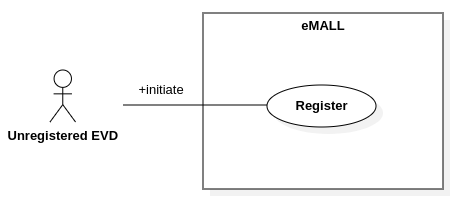
\includegraphics[width=0.9\linewidth]{Images/UseCaseDiagrams/unregistered_EVD_use_case_diagram}
        \caption{Unregistered EVD use case diagram.}
        \label{fig: unreg_EVD_diag}
    \end{center}
\end{figure}

\subsubsection*{Registered EVD}
\begin{figure} [H]
    \begin{center}
        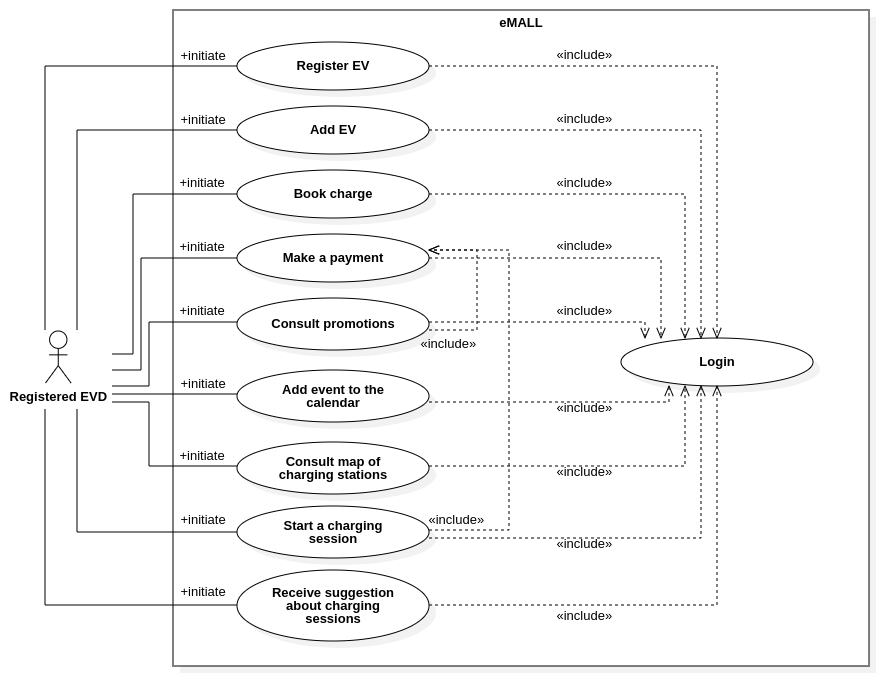
\includegraphics[width=0.9\linewidth]{Images/UseCaseDiagrams/registered_EVD_use_case_diagram}
        \caption{Unregistered EVD use case diagram.}
        \label{fig: reg_EVD_diag}
    \end{center}
\end{figure}

\subsubsection*{CPO}
\begin{figure} [H]
    \begin{center}
        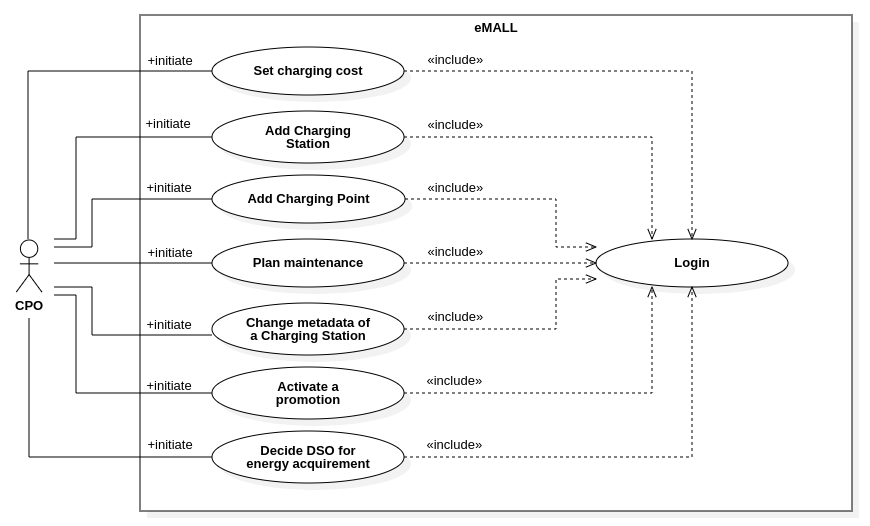
\includegraphics[width=0.9\linewidth]{Images/UseCaseDiagrams/CPO_use_case_diagram}
        \caption{Unregistered EVD use case diagram.}
        \label{fig: cpo_diag}
    \end{center}
\end{figure}

\subsection{Use cases}
\label{subsec: use_cases}%
\newcounter{uc}
\setcounter{uc}{1}
\newcommand{\cuc}{\theuc\stepcounter{uc}}
%TODO: write it better
In this section, they are explained and represented the main identified use cases.
There is a table with entry conditions, event flow, exit conditions and exception for each of them, and a sequence diagram
that shows the messages exchanged between the entities and the called functions. \\
%TODO: insert exeptions
\subsubsection*{UC\cuc . EVD signs up}
\begin{center}
    \begin{longtable}{lp{0.75\linewidth}}
        \hline
        Actor            & Unregistered EVD                                                                                                                                                                                       \\
        \hline
        Entry conditions & The EVD isn’t registered in the eMALL system, and he clicks the sign-up button                                                                                                                         \\
        \hline
        Event Flow       & 1.\ eMALL asks the unregistered EVD to insert personal information (i.e., name, surname, birthday, billing address, e-mail, and password).                                                             \\
        & 2.\ The unregistered EVD fills out the form with his personal information (name, surname, birthday, billing address, e-mail, and password) and accepts the “Terms \& Conditions” and “Privacy Policy”. \\
        & 3.\ eMALL validates the inserted EVD’s personal information.                                                                                                                                           \\
        & 4.\ eMALL asks the unregistered EVD to insert payment method information.                                                                                                                              \\
        & 5.\ The EVD fills out a form with its payment method information.                                                                                                                                      \\
        & 6.\ eMALL validates the inserted EVD’s payment method.                                                                                                                                                 \\
        & 7.\ eMALL sends a confirmation email to the EVD.                                                                                                                                                       \\
        & 8.\ eMALL sends back the EVD’s registration outcome.                                                                                                                                                   \\
        \hline
        Exit condition   & An account is created.                                                                                                                                                                                 \\
        \hline
        Exceptions       & 3.1. eMALL isn’t able to validate the EVD’s personal information.                                                                                                                                      \\
        & 6.1. eMALL isn’t able to validate the EVD’s payment method.                                                                                                                                            \\
        & In all these cases, the unregistered EVD is notified with an error message.                                                                                                                            \\
        \hline
        \caption{EVD signs up use case.}
        \label{tab: EVD_sign_up_use_case}
    \end{longtable}

        %TODO: insert sequence
        %\begin{figure} [H]
        %    \begin{center}
        %        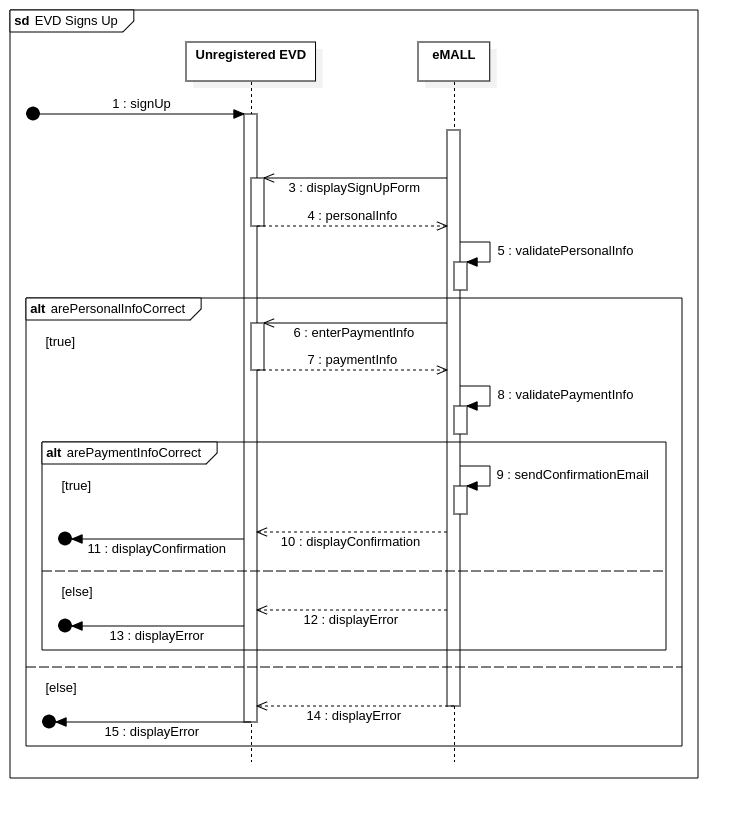
\includegraphics[width=0.9\linewidth]{Images/SequenceDiagrams/evd_signs_up}
        %        \caption{EVD signs up sequence diagram}
        %        \label{fig: evd_sign_up_seq_diag}
        %    \end{center}
        %\end{figure}
\end{center}

\subsubsection*{UC\cuc . Registered EVD logs in}
\begin{center}
    \begin{longtable}{lp{0.75\linewidth}}
        \hline
        Actor            & Registered EVD                                                                       \\
        \hline
        Entry conditions & The EVD is registered in the eMALL system and he clicks the log in button.           \\
        \hline
        Event Flow       & 1.\ eMALL asks the registered EVD to insert the e-mail.                              \\
        & 2.\ The registered EVD inserts the e-mail.                                           \\
        & 3.\ eMALL validates the inserted e-mail.                                             \\
        & 4.\ eMALL asks the registered EVD to insert the password associated with the e-mail. \\
        & 5.\ The registered EVD inserts the password.                                         \\
        & 6.\ eMALL validates the inserted password in combination with the e-mail.            \\
        & 7.\ eMALL sends back the login outcome.                                              \\
        \hline
        Exit condition   & The registered EVD access the eMALL system.                                          \\
        \hline
        Exceptions       & 3.1 The e-mail is not recognized.                                                    \\
        & 6.1 The password is not correct.                                                     \\
        & In both cases, the registered EVD receives a notification through an error message.
        He has to insert his credentials again. \\
        \hline
        \caption{Registered EVD logs in use case.}
        \label{tab: EVD_logs_in_use_case}
    \end{longtable}

        %TODO: insert sequence
        %\begin{figure} [H]
        %    \begin{center}
        %        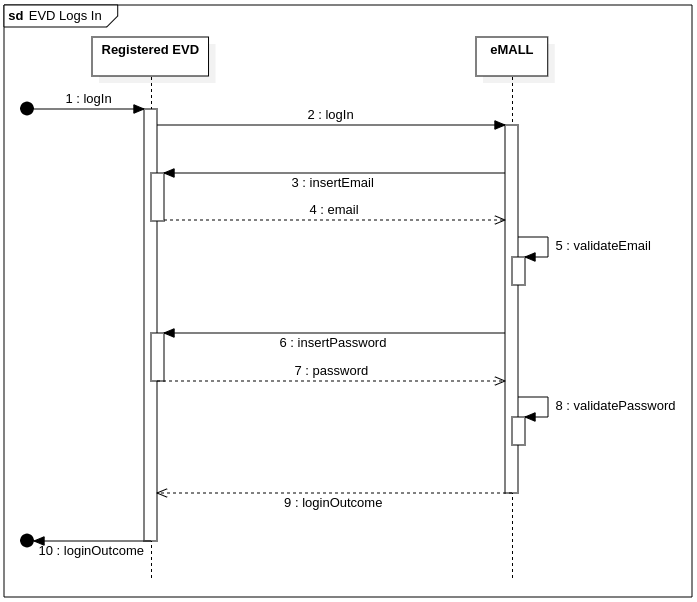
\includegraphics[width=0.9\linewidth]{Images/SequenceDiagrams/evd_logs_in}
        %        \caption{Registered EVD logs in sequence diagram}
        %        \label{fig: evd_logs_in_seq_diag}
        %    \end{center}
        %\end{figure}
\end{center}

\subsubsection*{UC\cuc . Registered EVD adds an EV}
\begin{center}
    \begin{longtable}{lp{0.75\linewidth}}
        \hline
        Actor            & Registered EVD                                                                                 \\
        \hline
        Entry conditions & The EVD is registered and correctly logged in.                                                 \\
        & The EVD clicks the ``Add a Vehicle'' button from his profile section of eMALL                  \\
        \hline
        Event Flow       & 1.\ eMALL asks the registered EVD to insert car information.                                   \\
        & 2.\ The registered EVD inserts the requested information and he sends them to the eMALL.       \\
        & 3.\ eMALL validates the information searching for possible errors.                             \\
        & 4.\ eMALL asks the registered EVD to insert a nickname for the vehicle to save in his profile. \\
        & 5.\ The registered EVD inserts the nickname.                                                   \\
        & 6.\ eMALL validates the nickname also searching for duplicates between user EV nicknames.      \\
        & 7.\ eMALL sends back the registration outcome.                                                 \\
        \hline
        Exit condition   & Registered EVD correctly added a new EV in the profile.                                        \\
        \hline
        Exceptions       & 3.1 The e-mail is not recognized.                                                              \\
        & 5.1 The inserted nickname is already taken between those owned by the user.                    \\
        & In both cases, the registered EVD receives a notification through an error message.            \\
        \hline
        \caption{Registered EVD adds an EV use case.}
        \label{tab: EVD_adds_a_vehicle_use_case}
    \end{longtable}

    \begin{figure} [H]
        \begin{center}
            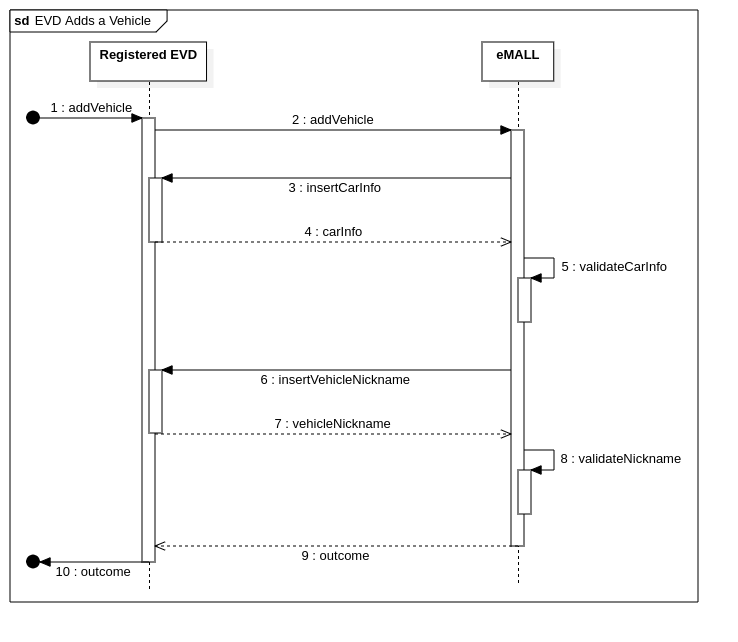
\includegraphics[width=0.9\linewidth]{Images/SequenceDiagrams/evd_adds_a_vehicle}
            \caption{Registered EVD adds an EV sequence diagram}
            \label{fig: evd_adds_ev_seq_diag}
        \end{center}
    \end{figure}
\end{center}

\subsubsection*{UC\cuc . Registered EVD books a charge}
\begin{center}
    \begin{longtable}{lp{0.75\linewidth}}
        \hline
        Actor            & Registered EVD                                                                                         \\
        \hline
        Entry conditions & The EVD is registered and correctly logged in.                                                         \\
        & The registered EVD selects a specific charging station and clicks the ``book'' button                  \\
        \hline
        Event Flow       & 1.\ eMALL asks the registered EVD to choose a timeframe.                                               \\
        & 2.\ The registered EVD inserts the timeframe.                                                          \\
        & 3.\ eMALL checks if the selected timeframe is currently available.                                     \\
        & 4.\ eMALL selects a charging point to reserve for the registered EVD depending on EV's specifications. \\
        & 5.\ eMALL asks the registered EVD to confirm the booking with the prompted information.                \\
        & 6.\ The registered EVD clicks the ``Confirm'' button to confirm the booking.                           \\
        & 7.\ eMALL adds the booking to the registered EVD's calendar.                                           \\
        & 8.\ eMALL sends back the booking outcome.                                                              \\
        \hline
        Exit condition   & A charging session is booked.                                                                          \\
        \hline
        Exceptions       & 3.1. No free charging points are available at the selected timeframe.                                  \\
        & The registered EVD is notified with an error message, and asked to select a new timeframe.             \\
        \hline
        \caption{Registered EVD books a charge use case.}
        \label{tab: EVD_booking_use_case}
    \end{longtable}

    \begin{figure} [H]
        \begin{center}
            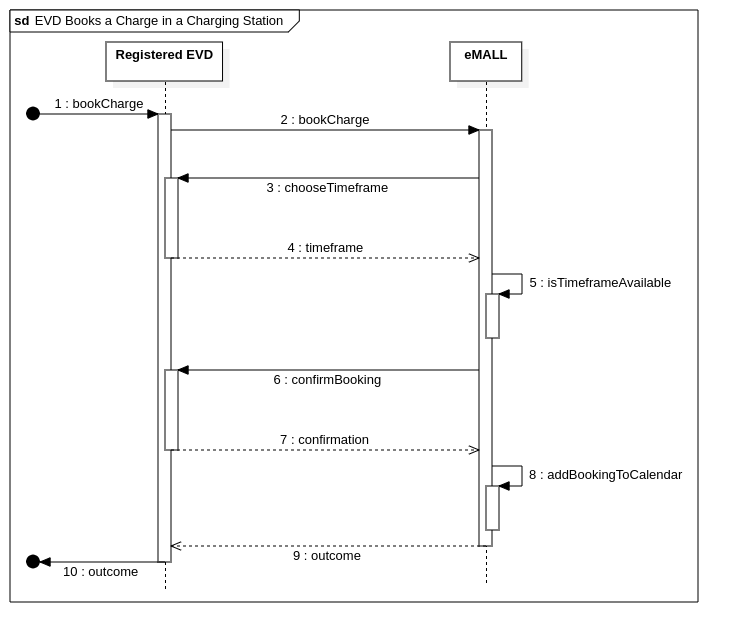
\includegraphics[width=0.9\linewidth]{Images/SequenceDiagrams/evd_books_a_charge_in_a_charging_station}
            \caption{Registered EVD books a charge sequence diagram}
            \label{fig: evd_books_charge_seq_diag}
        \end{center}
    \end{figure}
\end{center}

\subsubsection*{UC\cuc . Registered EVD consults the map of charging stations}
\begin{center}
    \begin{longtable}{lp{0.75\linewidth}}
        \hline
        Actor            & Registered EVD                                                                                               \\
        \hline
        Entry conditions & The EVD is registered and correctly logged in.                                                               \\
        & The registered EVD is in the map section at a given or specified location.                                   \\
        \hline
        Event Flow       & 1.\ eMALL shows the map with all the charging stations available over a specific location.                   \\
        & 2.\ The registered EVD moves on the map, searching for a charging station.                                   \\
        & 3.\ eMALL retrieves the charging station locations in the new place.                                         \\
        & 4.\ The registered EVD selects a specific charging station to get its detailed information.                  \\
        & 5.\ eMALL retrieves the charging station's detailed information.                                             \\
        \hline
        Exit condition   & The registered EVD changes section, and moves from the dashboard.                                            \\
        \hline
        Exceptions       & 1.1 The registered EVD did not accept sharing location.                                                      \\
        & In this case, the registered EVD is notified by an error message and needs to move to its position manually. \\
        \hline
        \caption{Registered EVD consults the map of charging stations use case.}
        \label{tab: EVD_map_charging_stations_use_case}
    \end{longtable}

    \begin{figure} [H]
        \begin{center}
            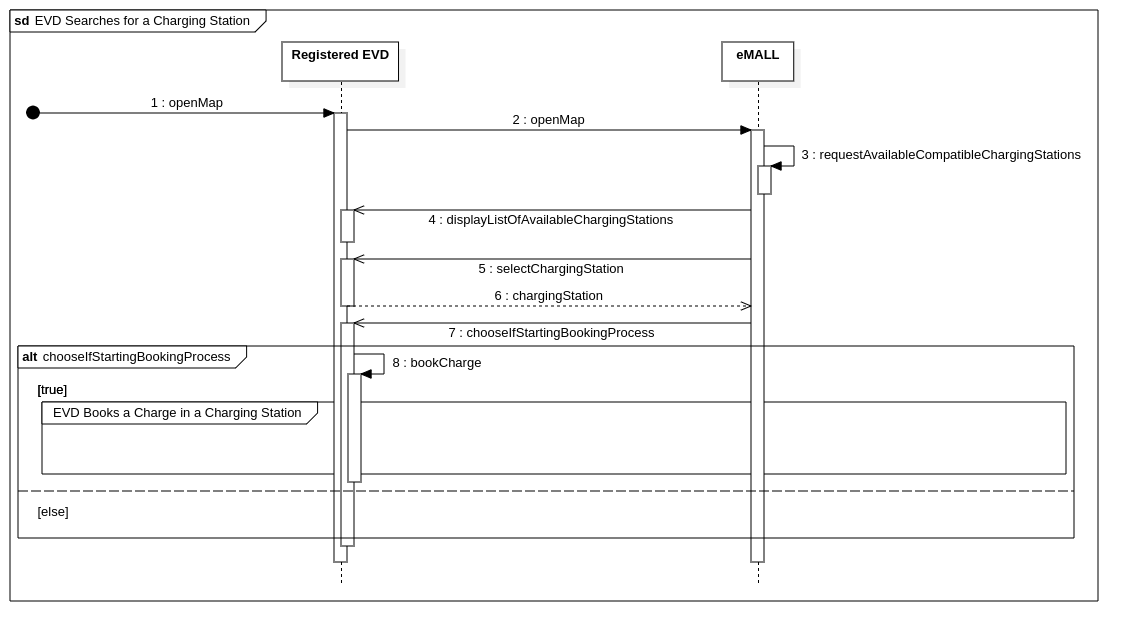
\includegraphics[width=0.9\linewidth]{Images/SequenceDiagrams/evd_searches_for_a_charging_station}
            \caption{Registered EVD consults the map of charging stations sequence diagram}
            \label{fig: evd_consults_stations_seq_diag}
        \end{center}
    \end{figure}
\end{center}

\subsubsection*{UC\cuc . Registered EVD consults a specific promotion that can be redeemed}
\begin{center}
    \begin{longtable}{lp{0.75\linewidth}}
        \hline
        Actor            & Registered EVD                                                                                                        \\
        \hline
        Entry conditions & The EVD is registered and correctly logged in.                                                                        \\
        & The EVD is in the promotion section.                                                                                  \\
        \hline
        Event Flow       & 1.\ eMALL sends the promotion list to the registered EVD.                                                             \\
        & 2.\ The registered EVD selects a promotion to activate.                                                               \\
        & 3.\ The registered EVD triggers the offer.                                                                            \\
        & 4.\ eMALL asks the registered EVD to choose between his payment methods.                                              \\
        & 5.\ The registered EVD picks the payment method.                                                                      \\
        & 6.\ eMALL asks the registered EVD to confirm the payment.                                                             \\
        & 7.\ The registered EVD authorizes the payment.                                                                        \\
        & 8.\ eMALL makes the payment.                                                                                          \\
        & 9.\ eMALL sends back the payment outcome.                                                                             \\
        \hline
        Exit condition   & The promotion has been activated.                                                                                     \\
        \hline
        Exceptions       & 8.1. The payment fails due to no sufficient funds.                                                                    \\
        & 8.2. The payment fails due to the failure of the transaction.                                                         \\
        & 8.3. The payment fails because of data input errors.                                                                  \\
        & 8.4. The payment fails due to technical issues.                                                                       \\
        & In these cases, the registered EVD receives a notification with an error message, and the promotion is not activated. \\
        \hline
        \caption{Registered EVD consults a specific promotion that can be redeemed use case.}
        \label{tab: EVD_consults_promotion_use_case}
    \end{longtable}

    \begin{figure} [H]
        \begin{center}
            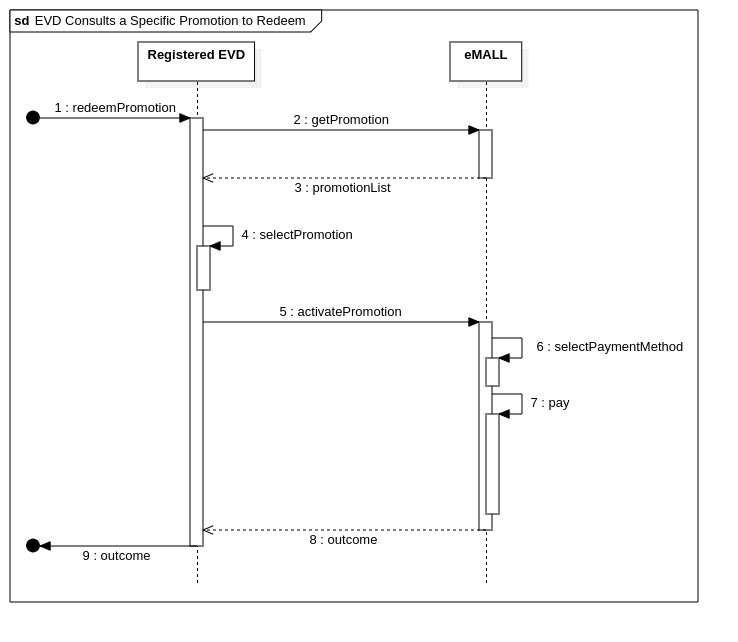
\includegraphics[width=0.9\linewidth]{Images/SequenceDiagrams/evd_consults_a_specific_promotion_to_redeem}
            \caption{Registered EVD consults a specific promotion that can be redeemed sequence diagram}
            \label{fig: evd_consults_promotion_seq_diag}
        \end{center}
    \end{figure}
\end{center}

\subsubsection*{UC\cuc . Registered EVD starts the charging process}
\begin{center}
    \begin{longtable}{lp{0.75\linewidth}}
        \hline
        Actor            & Registered EVD                                                                                                       \\
        \hline
        Entry conditions & The EVD is registered and correctly logged in.                                                                       \\
        & The EVD starts charging the EV at a charging point of the charging station.                                          \\
        \hline
        Event Flow       & 1.\ eMALL communicates to the EVD if he has been correctly authenticated and if he can charge at the charging point. \\
        & 2.\ The registered EVD initializes the charging process.                                                             \\
        & 3.\ eMALL defines the source of the electricity (batteries or DSO).                                                  \\
        & 4.\ eMALL defines how much electricity to give to the connected EV depending on actual energy demand.                \\
        & 5.\ eMALL sends updates of the charging session to the EVD.                                                          \\
        & 6.\ The registered EVD stops the charging process.                                                                   \\
        & 7.\ eMALL sends the receipt of the charging session to the EVD.                                                      \\
        & 8.\ The registered EVD makes the payment for the charging session.                                                   \\
        & 9.\ eMALL sends back the payment outcome                                                                             \\
        \hline
        Exit condition   & The registered EVD has charged the EV and paid for the service received.                                             \\
        \hline
        Exceptions       &                                                                                                                      \\
        \hline
        \caption{Registered EVD starts the charging process use case.}
        \label{tab: EVD_charges_EV_use_case}
    \end{longtable}

        %TODO: insert sequence
        %\begin{figure} [H]
        %    \begin{center}
        %        \includegraphics[width=0.9\linewidth]{Images/SequenceDiagrams/evd_starts_charging}
        %        \caption{Registered EVD starts the charging process sequence diagram}
        %        \label{fig: evd_starts_charging_seq_diag}
        %    \end{center}
        %\end{figure}
\end{center}

\subsubsection*{UC\cuc . Registered EVD makes a payment}
\begin{center}
    \begin{longtable}{lp{0.75\linewidth}}
        \hline
        Actor            & Registered EVD                                                                                                        \\
        \hline
        Entry conditions & The EVD is registered and correctly logged in.                                                                        \\
        & The registered EVD has decided the charging station where will charge the EV and is in the payment module.            \\
        \hline
        Event Flow       & 1.\ eMALL shows registered EVD's payment methods and asks to select one of them.                                      \\
        & 2.\ The registered EVD selects a payment method.                                                                      \\
        & 3.\ eMALL verifies funds availability.                                                                                \\
        & 4.\ eMALL starts the payment process.                                                                                 \\
        & 5.\ eMALL sends back the payment outcome.                                                                             \\
        \hline
        Exit condition   & The registered EVD has paid for a book or for a activation of a promotion.                                            \\
        \hline
        Exceptions       & 5.1. The payment fails due to no sufficient funds.                                                                    \\
        & 5.2. The payment fails due to the failure of the transaction.                                                         \\
        & 5.3. The payment fails because of data input errors.                                                                  \\
        & 5.4. The payment fails due to technical issues.                                                                       \\
        & In these cases, the registered EVD receives a notification with an error message, and the promotion is not activated. \\
        \hline
        \caption{Registered EVD makes a payment use case.}
        \label{tab: EVD_pays_use_case}
    \end{longtable}

    \begin{figure} [H]
        \begin{center}
            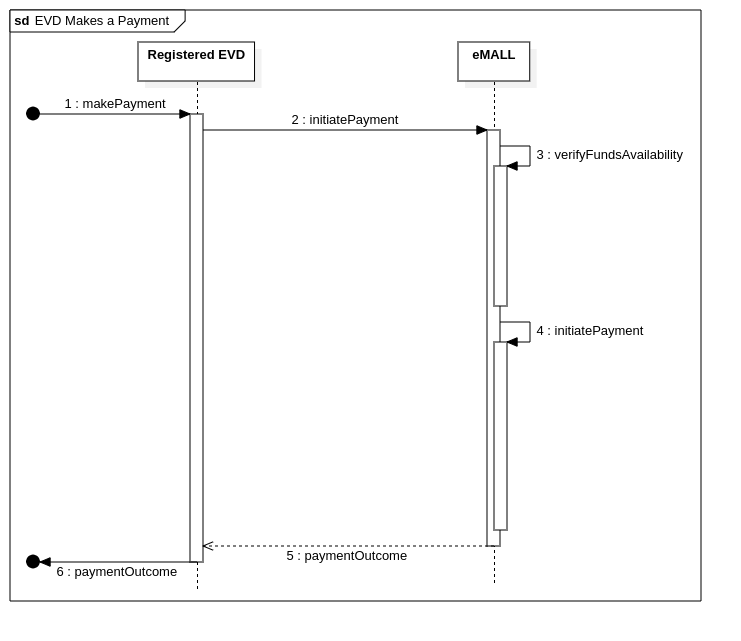
\includegraphics[width=0.9\linewidth]{Images/SequenceDiagrams/evd_makes_a_payment}
            \caption{Registered EVD makes a payment sequence diagram}
            \label{fig: evd_pays_seq_diag}
        \end{center}
    \end{figure}
\end{center}

\subsubsection*{UC\cuc . Registered EVD adds a new activity into the calendar and receives suggestions about charging schedule}
\begin{center}
    \begin{longtable}{lp{0.75\linewidth}}
        \hline
        Actor            & Registered EVD                                                                                                \\
        \hline
        Entry conditions & The EVD is registered and correctly logged in.                                                                \\
        & The registered EVD opens the calendar section.                                                                \\
        \hline
        Event Flow       & 1.\ eMALL shows the calendar to the registered EVD.                                                           \\
        & 2.\ The registered EVD clicks the ``insert new activity'' button.                                             \\
        & 3.\ eMALL sends the form to be compiled for the addition of a new activity.                                   \\
        & 4.\ The registered EVD inserts and submits the requested information.                                         \\
        & 5.\ eMALL processes the received form.                                                                        \\
        & 6.\ eMALL saves the new activity into registered EVD calendar.                                                \\
        & 7.\ eMALL calculates the best schedule of where and when to charge the EV and sends it to the registered EVD. \\
        & 8.\ The registered EVD selects a charging station from the list of stations suggested by \verb|eMALL|.        \\
        & 9.\ eMALL books the selected charging station at the specified timeframe.                                     \\
        & 10.\ eMALL sends back the booking outcome to the registered EVD.                                              \\
        \hline
        Exit condition   & The registered EVD inserted a new activity received a suggestion about charging session.                      \\
        \hline
        Exceptions       &                                                                                                               \\
        \hline
        \caption{Registered EVD adds a new activity into the calendar and receives suggestions about charging schedule use case.}
        \label{tab: EVD_adds_activity_calendar_use_case}
    \end{longtable}

    \begin{figure} [H]
        \begin{center}
            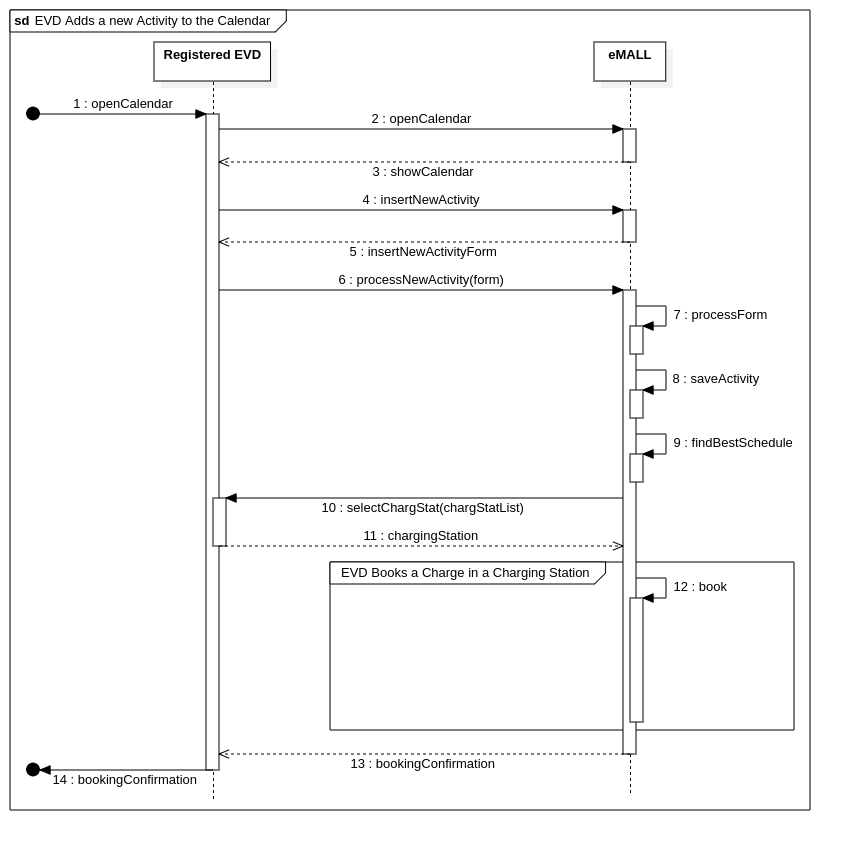
\includegraphics[width=0.9\linewidth]{Images/SequenceDiagrams/evd_adds_a_new_activity_to_the_calendar}
            \caption{Registered EVD adds a new activity into the calendar and receives suggestions about charging schedule sequence diagram}
            \label{fig: evd_adds_activity_seq_diag}
        \end{center}
    \end{figure}
\end{center}

\subsubsection*{UC\cuc . CPO logs in}
\begin{center}
    \begin{longtable}{lp{0.75\linewidth}}
        \hline
        Actor            & CPO                                                                                                 \\
        \hline
        Entry conditions & CPO’s operator is in the business login section.                                                    \\
        \hline
        Event Flow       & 1.\ eMALL asks the CPO operator to insert his credentials to log in.                                \\
        & 2.\ The CPO operator inserts the CPO ID associated with its company, password, and email.           \\
        & 3.\ eMALL validates the inserted credentials combination.                                           \\
        & 4.\ eMALL sends back the login outcome.                                                             \\
        \hline
        Exit condition   & The CPO access the business section of the eMALL system                                             \\
        \hline
        Exceptions       & 3.1.1. CPO credentials are not correct and not validated by eMALL.                                  \\
        & 3.2.1. CPO’s affiliate agreement has expired, and its ID is no longer allowed to access the system. \\
        & In both cases, the user receives a notification with an error message.                              \\
        & Also, in the second case, the operator is invited to call the sales team.                           \\
        \hline
        \caption{CPO logs in use case.}
        \label{tab: CPO_logs_in_use_case}
    \end{longtable}

        %TODO: add sequence diagram
        %\begin{figure} [H]
        %    \begin{center}
        %        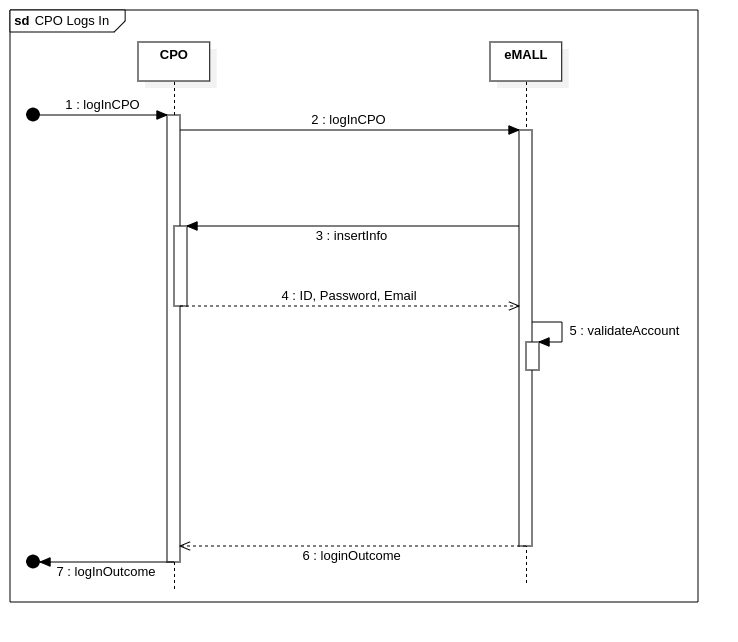
\includegraphics[width=0.9\linewidth]{Images/SequenceDiagrams/cpo_logs_in}
        %        \caption{CPO logs in sequence diagram}
        %        \label{fig: cpo_log_in_seq_diag}
        %    \end{center}
        %\end{figure}
\end{center}

\subsubsection*{UC\cuc . CPO sets the charging cost}
\begin{center}
    \begin{longtable}{lp{0.75\linewidth}}
        \hline
        Actor            & CPO                                                                \\
        \hline
        Entry conditions & The CPO is subscribed to the eMALL system and correctly logged in. \\
        & The CPO enters the profile section.                                \\
        \hline
        Event Flow       & 1.\ eMALL shows the CPO his profile.                               \\
        & 2.\ The CPO enters the charging station managing section.          \\
        & 3.\ eMALL shows the CPO his managing charging station section.     \\
        & 4.\ The CPO taps the ``manage price'' button.                      \\
        & 5.\ The CPO inserts the value of the fee.                          \\
        & 6.\ The CPO taps the submission button.                            \\
        & 7.\ eMALL sends back the outcome of the setting of the fee.        \\
        \hline
        Exit condition   & The fee is set to the new value.                                   \\
        \hline
        Exceptions       &                                                                    \\
        \hline
        \caption{CPO sets a fee use case.}
        \label{tab: CPO_sets_fee_use_case}
    \end{longtable}

    \begin{figure} [H]
        \begin{center}
            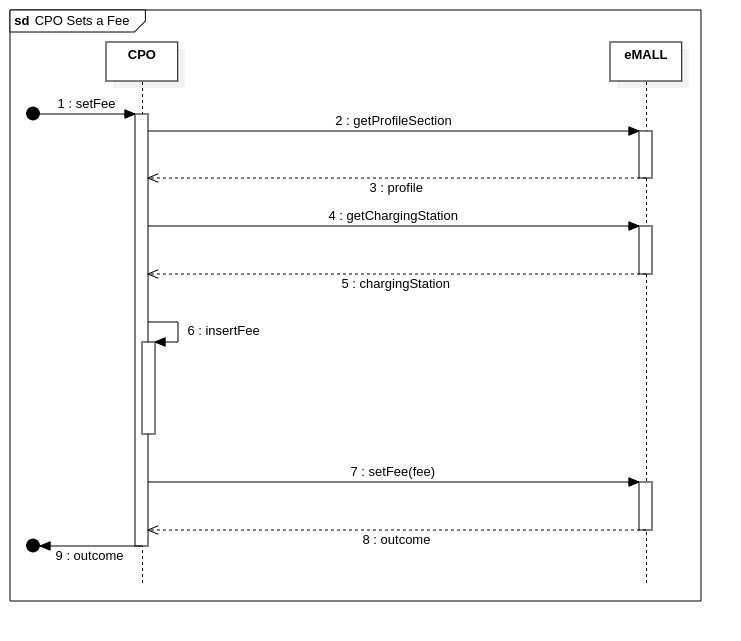
\includegraphics[width=0.9\linewidth]{Images/SequenceDiagrams/cpo_sets_a_fee}
            \caption{CPO sets a fee sequence diagram}
            \label{fig: cpo_sets_fee_seq_diag}
        \end{center}
    \end{figure}
\end{center}

\subsubsection*{UC\cuc . CPO adds a charging station}
\begin{center}
    \begin{longtable}{lp{0.75\linewidth}}
        \hline
        Actor            & CPO                                                                                                       \\
        \hline
        Entry conditions & The CPO is subscribed to the eMALL system and correctly logged in.                                        \\
        & The CPO is in the charging station section from the profile section.                                      \\
        & The CPO clicks the button to add a new charging station to its profile.                                   \\
        \hline
        Event Flow       & 1.\ eMALL asks the CPO to insert the location of the new charging station.                                \\
        & 2.\ The CPO inserts the region, province, city, and address of the new charging station.                  \\
        & 3.\ eMALL asks the CPO to insert the initial status of the new charging station.                          \\
        & 4.\ The CPO inserts the status of the new charging station (available, maintenance, broken, unavailable). \\
        & 5.\ eMALL asks the CPO to insert the charging costs.                                                      \\
        & 6.\ The CPO inserts the charging costs.                                                                   \\
        & 7.\ eMALL asks the CPO to add charging points to the new charging station.                                \\
        & 8.\ The CPO inserts the information of the charging points.                                               \\
        & 9.\ eMALL validates all the inserted information.                                                         \\
        & 10.\ eMALL sends back the outcome of the insertion of the new charging station.                           \\
        \hline
        Exit condition   & The charging station is created and added to the CPO’s profile.                                           \\
        \hline
        Exceptions       & 9.1 There is already a charging station at the same location specified by the CPO.                        \\
        & The CPO receives a notification with an error message, and the charging station is not created.           \\
        \hline
        \caption{CPO adds a charging station use case.}
        \label{tab: CPO_adds_charging_station_use_case}
    \end{longtable}

    \begin{figure} [H]
        \begin{center}
            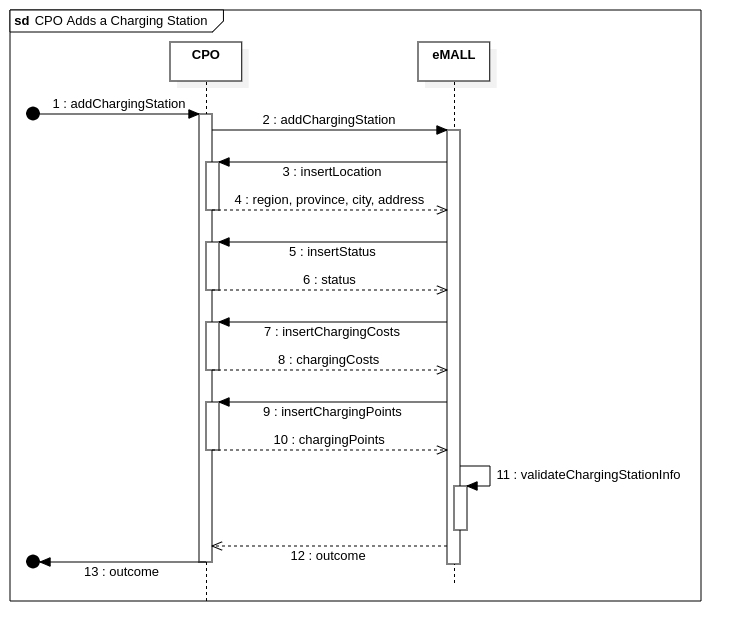
\includegraphics[width=0.9\linewidth]{Images/SequenceDiagrams/cpo_adds_a_charging_stations}
            \caption{CPO adds a charging station sequence diagram}
            \label{fig: cpo_adds_station_seq_diag}
        \end{center}
    \end{figure}
\end{center}

\subsubsection*{UC\cuc . CPO adds a charging point}
\begin{center}
    \begin{longtable}{lp{0.75\linewidth}}
        \hline
        Actor            & CPO                                                                                             \\
        \hline
        Entry conditions & The CPO is subscribed to the eMALL system and correctly logged in.                              \\
        & The CPO is in the charging station section from the profile section.                            \\
        & The CPO clicks the “add charging point” button.                                                 \\
        \hline
        Event Flow       & 1.\ eMALL shows the CPO the list of its charging stations and asks it to select one.            \\
        & 2.\ The CPO selects a charging station.                                                         \\
        & 3.\ eMALL asks the CPO to insert the information about the charging station.                    \\
        & 4.\ The CPO inserts the serial number, the types of connectors installed on the charging point, the power supply,
        the initial status of the charging point, and the other required information. \\
        & 5.\ eMALL validates the inserted information about the charging point.                          \\
        & 6.\ eMALL sends back to the CPO the outcome of the creation of the new charging point.          \\
        \hline
        Exit condition   & The charging point is added to the charging station.                                            \\
        \hline
        Exceptions       & 4.1 There is already a charging point with the same serial number in the profile of the CPO.    \\
        & The CPO receives a notification with an error message, and the charging station is not created. \\
        \hline
        \caption{CPO adds a charging point use case.}
        \label{tab: CPO_adds_charging_point_use_case}
    \end{longtable}

    \begin{figure} [H]
        \begin{center}
            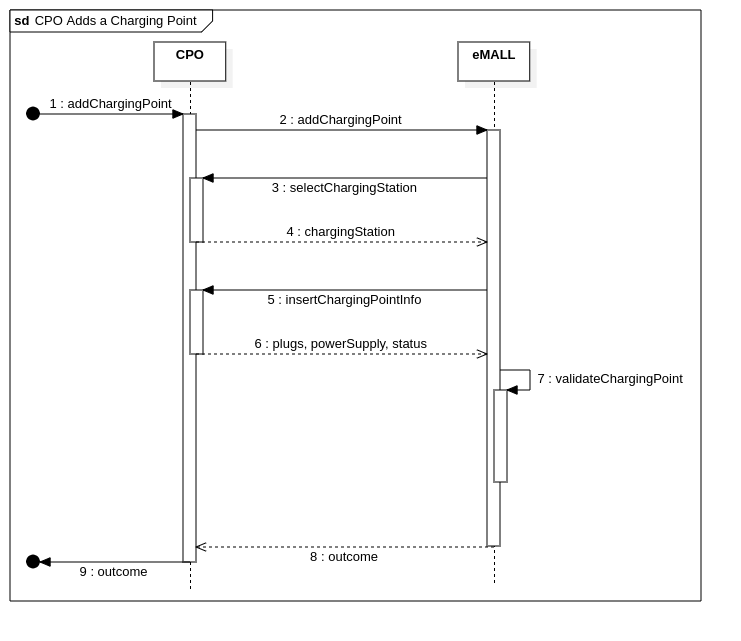
\includegraphics[width=0.9\linewidth]{Images/SequenceDiagrams/cpo_adds_a_charging_point}
            \caption{CPO adds a charging point sequence diagram}
            \label{fig: cpo_adds_point_seq_diag}
        \end{center}
    \end{figure}
\end{center}

\subsubsection*{UC\cuc . CPO changes the metadata of a charging point}
\begin{center}
    \begin{longtable}{lp{0.75\linewidth}}
        \hline
        Actor            & CPO                                                                                  \\
        \hline
        Entry conditions & The CPO is subscribed to the eMALL system and correctly logged in.                   \\
        & The CPO is in the charging station section from the profile section.                 \\
        & The CPO clicks the “edit charging station” button.                                   \\
        \hline
        Event Flow       & 1.\ eMALL shows the CPO the list of its charging stations and asks it to select one. \\
        & 2.\ The CPO selects a charging station.                                              \\
        & 3.\ eMALL asks the CPO to insert the new values for the charging point.              \\
        & 4.\ The CPO edits the metadata of the charging station.                              \\
        & 5.\ eMALL updates the charging point with the new inserted values.                   \\
        & 6.\ eMALL sends back to the CPO the outcome of the update.                           \\
        \hline
        Exit condition   & The metadata of the charging station is updated.                                     \\
        \hline
        Exceptions       &                                                                                      \\
        \hline
        \caption{CPO changes the metadata of a charging point use case.}
        \label{tab: CPO_updates_charging_point_use_case}
    \end{longtable}

    \begin{figure} [H]
        \begin{center}
            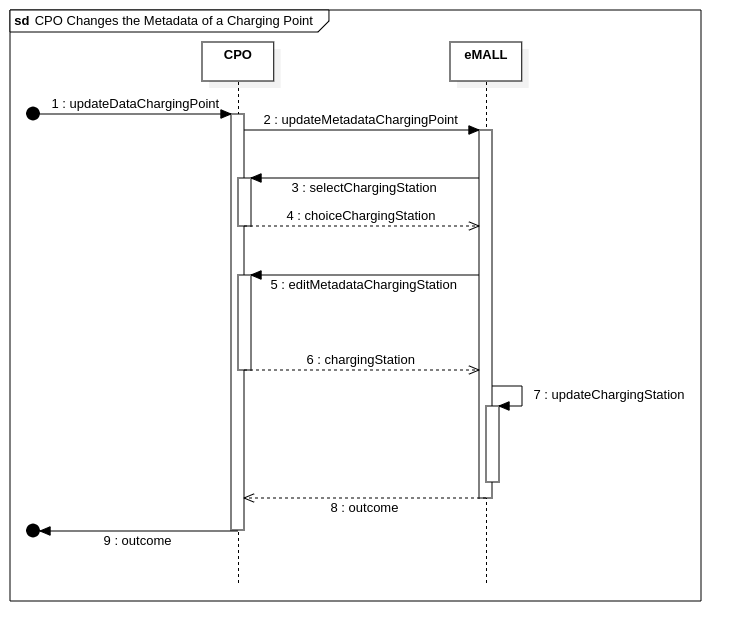
\includegraphics[width=0.9\linewidth]{Images/SequenceDiagrams/cpo_changes_the_metadata_of_a_charging_point}
            \caption{CPO changes the metadata of a charging point sequence diagram}
            \label{fig: cpo_updates_metadata_point_seq_diag}
        \end{center}
    \end{figure}
\end{center}

\subsubsection*{UC\cuc . CPO activates a promotion}
\begin{center}
    \begin{longtable}{lp{0.75\linewidth}}
        \hline
        Actor            & CPO                                                                                 \\
        \hline
        Entry conditions & The CPO is subscribed to the eMALL system and correctly logged in.                  \\
        & The CPO is in the profile section.                                                  \\
        & The CPO clicks the “activate new promotion” button.                                 \\
        \hline
        Event Flow       & 1.\ eMALL asks the CPO to define the features of the new promotion.                 \\
        & 2.\ The CPO defines the features of the new promotion.                              \\
        & 3.\ eMALL saves the new promotion.                                                  \\
        & 4.\ eMALL initializes the promotion.                                                \\
        & 5.\ eMALL sends back to the CPO the outcome of the activation of the new promotion. \\
        \hline
        Exit condition   & The promotion is created and activated.                                             \\
        \hline
        Exceptions       &                                                                                     \\
        \hline
        \caption{CPO activates a promotion use case.}
        \label{tab: CPO_activates_promotion_use_case}
    \end{longtable}

    \begin{figure} [H]
        \begin{center}
            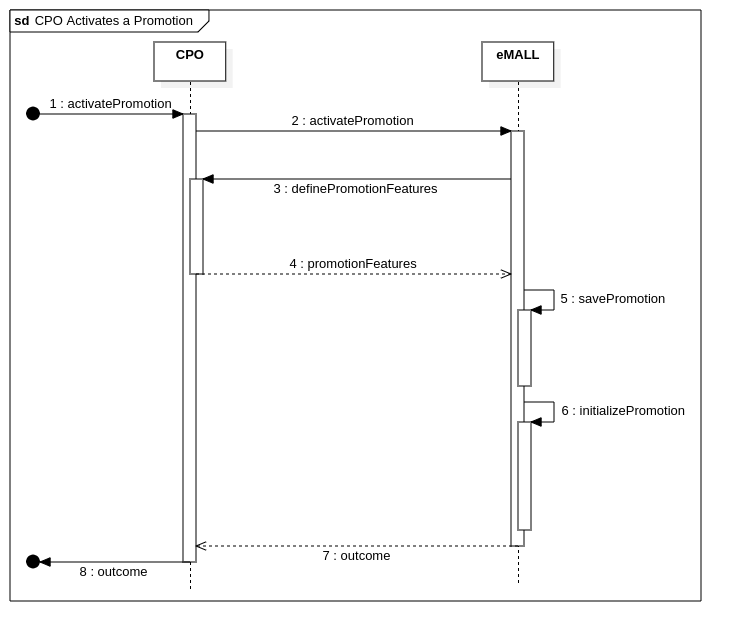
\includegraphics[width=0.9\linewidth]{Images/SequenceDiagrams/cpo_activates_a_promotion}
            \caption{CPO activates a promotion sequence diagram}
            \label{fig: cpo_activate_promo_seq_diag}
        \end{center}
    \end{figure}
\end{center}

\subsubsection*{UC\cuc . CPO plans a maintenance session for a charging station}
\begin{center}
    \begin{longtable}{lp{0.75\linewidth}}
        \hline
        Actor            & CPO                                                                                             \\
        \hline
        Entry conditions & The CPO is subscribed to the eMALL system and correctly logged in.                              \\
        & The CPO is in the charging station section from the profile section and has selected a station. \\
        & The CPO clicks the ``schedule maintenance'' button.                                             \\
        \hline
        Event Flow       & 1.\ eMALL asks the CPO to specify the date and the hour of the maintenance.                     \\
        & 2.\ eMALL plans the maintenance session of the charging station.                                \\
        & 3.\ eMALL sends back the outcome of the planning of the maintenance to the CPO.                 \\
        \hline
        Exit condition   & It is planned a maintenance session for the specified charging station.                         \\
        \hline
        Exceptions       &                                                                                                 \\
        \hline
        \caption{CPO plans a maintenance session for a charging station use case.}
        \label{tab: CPO_plans_maintenance_use_case}
    \end{longtable}

        %TODO: add sequence diagram
        %\begin{figure} [H]
        %    \begin{center}
        %        \includegraphics[width=0.9\linewidth]{Images/SequenceDiagrams/cpo_plans_maintenance}
        %        \caption{CPO plans a maintenance session for a charging station sequence diagram}
        %        \label{fig: cpo_plans_maintenance_seq_diag}
        %    \end{center}
        %\end{figure}
\end{center}

\subsubsection*{UC\cuc . CPO decides the DSO from which acquire energy}
\begin{center}
    \begin{longtable}{lp{0.75\linewidth}}
        \hline
        Actor            & CPO                                                                           \\
        \hline
        Entry conditions & The CPO is subscribed to the eMALL system and correctly logged in.            \\
        & The CPO is in the DSO section from the profile section.                       \\
        & The CPO clicks the “set DSO” button.                                          \\
        \hline
        Event Flow       & 1.\ eMALL shows the CPO the list of DSOs.                                     \\
        & 2.\ eMALL asks the CPO to select a DSO from the list.                         \\
        & 3.\ The CPO selects a DSO from the list.                                      \\
        & 4.\ eMALL updates CPO’s profile information.                                  \\
        & 5.\ eMALL activates the selected DSO as the one from which to acquire energy. \\
        & 6.\ eMALL sends back to the CPO the outcome of the setting of the DSO         \\
        \hline
        Exit condition   & The DSO from which to acquire energy is updated.                              \\
        \hline
        Exceptions       &                                                                               \\
        \hline
        \caption{CPO decides the DSO from which acquire energy use case.}
        \label{tab: CPO_decides_DSO_use_case}
    \end{longtable}

    \begin{figure} [H]
        \begin{center}
            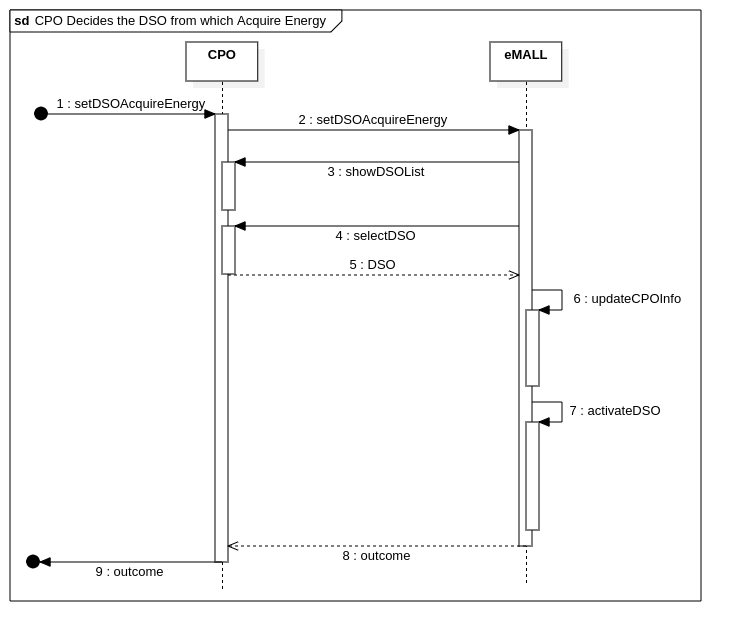
\includegraphics[width=0.9\linewidth]{Images/SequenceDiagrams/cpo_decides_the_dso_from_which_acquire_energy}
            \caption{CPO decides the DSO from which acquire energy sequence diagram}
            \label{fig: cpo_decides_DSO_seq_diag}
        \end{center}
    \end{figure}
\end{center}

\subsection{Mapping on requirements}
\label{subsec: map_on_req}%
\newcounter{mr}
\setcounter{mr}{1}
\newcommand{\cmr}{\themr\stepcounter{mr}}
\begin{center}
    \begin{longtable}{|l|l|}
        \hline
        \textbf{Use Case} & \textbf{Requirements} \\
        \hline
        \caption{Mapping on requirements.}
        \label{tab: map_on_req}
    \end{longtable}
\end{center}


\section{Performance Requirements}
\label{sec:performance_requirements}%
\subsection*{Number of users}
According to a market analysis conducted by \verb|MOTUS-E| in September 2022,
the number of fully electric vehicles and plug-in hybrid vehicles registered in Italy is 320.776.
If we suppose that the eMALL system will be used by one in every three EVDs,
the system should guarantee that it can handle an overall of 100.000 clients. \\
So, we can consider that the system should be able to handle th $50\%$ of them could be connected simultaneously.

\subsection*{Data storage}
From the data storage point of view, the \verb|eMALL| system should consider several sources of data:
\begin{itemize}
    \item \textbf{EVD's personal data.} We consider that $5\ KB$ is enough for the storage of personal information of an EVD\@.
    Considering $10^5$ EVDs, the system needs:
    \[
        10^5 \cdot 5\ KB = 488,3\ MB
    \]
    \item \textbf{EVD's calendar.} One of the functionalities offered by the \verb|eMALL| system is to insert new activities
    into EVD's calendar.
    The events have not much information: they specify starting time and destination of the activity.
    We can assume that each event requires $1 KB$ of storage.
    Considering all the potential users and assuming that they insert three activities a day, for the first year the system needs:
    \[
        10^5\cdot 3\cdot 365\cdot 1\ KB = 104,43\ GB
    \]
    \item \textbf{History of charging sessions.} The \verb|eMALL| system should save the information of all the charging sessions.
    We assume that the information of each charging session requires $3\ KB$ of storage.
    To decide how many times we want to assume a generic EVD charges his EV, we have to consider different factors,
    such as the EVDs' habits, the storage of their EV's battery, and the distances they can drive during the day.
    For example, an EVD who drives long distances every day and whose EV has a small battery may need to charge
    it more frequently than an EVD with a larger battery who only drives short distances.
    Similarly, an EVD that can access fast charging infrastructure may be able to charge his EV less frequently than
    a driver who only has access to slower charging stations.
    So, it is reasonable to assume that a generic EVD charges his EV twice a week. \\
    For the first year, the system needs:
    \[
        10^5 \cdot \frac{365}{7} \cdot 2 \cdot 3\ KB = 29,84\ GB
    \]
    \item \textbf{CPO's personal data.} If we consider that in Italy there could be more or less 50 CPOs,
    as we did for the EVDs, we can assume that one in every three CPOs subscribes to the \verb|eMALL| system.
    We consider enough $5\ KB$ of storage for each profile.
    So, the system needs:
    \[
        20 \cdot 5\ KB = 100\ KB
    \]
    \item \textbf{Charging points registration.} Each CPO registers information about their charging points distributed in the territory.
    Referring again to the market analysis conducted by \verb|MOTUS-E|, in September 2022,
    there were a total of 32.776 charging points in Italy.
    So, we can assume that all the CPOs register 11.000 charging points all together.
    We consider enough $5\ KB$ of storage for the registration of each charging spot.
    So, the system needs:
    \[
        11 000 \cdot 5\ KB = 53,71\ MB
    \]
\end{itemize}
The rest of storage needed is about the several functionalities offered to the EVDs and to the CPOs.
So, after summing all the values obtained in the previous list, we overestimate the memory suggested for the first year
of life of the system.
Summing all the values, it is:
\[
    488,3\ MB + 104,43\ GB + 29,84\ GB + 100\ KB + 53,71\ MB = 134,8\ GB
\]
So, a memory storage of $200\ GB$ will be enough for the first year of the \verb|eMALL| system.

\textbf{Time response} \\
The \verb|eMALL| system should handle all the requests within 3 seconds, given that there are not strict time response requirements.


\section{Design Constraints}
\label{sec:design_constraints}%

\subsection{Standards compliance}
\label{subsec:standards_compliance}%
First of all, the system should respect all the laws regarding privacy and data treatment and exchange with third parties (i.e.\ CPOs);
to work in Europe, the system should respect the EU GDPR\@.
In particular, a general description of the main principles that data should have in order to guarantee their privacy
is given in Art.\ 5 of the GDPR document.

\subsection{Hardware limitations}
\label{subsec:hardware_limitations}%
The \verb|eMALL| system can be used from both web browsers and mobile applications.
As explained in the system attributes section, the system is strictly related to the operating systems
in which the mobile application will be implemented, so Android and IO\@..

\subsection{Any other constraint}
\label{subsec:any_other_constraint}%
There are not other constraints.


\section{Software System Attributes}
\label{sec:software_system_attributes}%

\subsection{Reliability}
\label{subsec:reliability}%
The \verb|eMALL| system should guarantee critical operations as payment.
But, its functionalities are mainly about data management of the user and CPOs' infrastructure.
It would not be critical if one of these operations fails, given that the process can be started and repeated.
So, considering the different behaviors the system should have, it is reasonable to have a failure rate
between $0.1\%$ and $1\%$, so to be between high-quality reliable systems and more common systems.

\subsection{Availability}
\label{subsec:availability}%
The \verb|eMALL| system should guarantee the CPO a good experience in their IT infrastructure management.
So, considering the business functionalities that the system offers to the companies, it would not be acceptable a day of downtime.
That's the reason why the system should guarantee $99.9\%$ of uptime.
In this section we just consider the business functionalities because the interactions between the EVDs and \verb|eMALL|
don't introduce constraints for the availability of the system.

\subsection{Security}
\label{subsec:security}%
The \verb|eMALL| system communicates with EVDs and CPOs, and stores their personal information.
For this reason, it should assure data privacy and data encryption when information is exchanged through the internet.
This is guaranteed thanks to the HTTPS\@.
Furthermore, \verb|eMALL| should encrypt all the information before proceeding with the storage.

\subsection{Maintainability}
\label{subsec:maintainability}%
The \verb|eMALL| system should be divided in different modules depending on the offered functionalities.
It is necessary to facilitate maintenance and substitution of the modules, and to eventually extend the system.
Furthermore, every implemented functionality has to be well documented.
What should guide the design definition process is to allow a maintenance that does not affect untouched modules and their interfaces.

\subsection{Portability}
\label{subsec:portability}%
The \verb|eMALL| system is not strictly related to software and hardware.
To be more portable, the system can be developed on both Android and IOS\@.
In order to do that, it has to be decided which programming language and development tools to use:
if the budget is not high and would be better to save time and effort, it is recommended to use cross-platform
development tools;
otherwise, the system can be implemented separately,
increasing in that way the effort needed for the developing and the maintenance of the applications.